\index{Kuzmann, Ute}

\paragraph{Research Team}
Ute Kunzmann (Professor), Caroline Schuster Cordone (Doctoral Candidate (University of Fribourgh, Switzerland).

 This project deals with a research topic that transcends disciplinary boundaries. Funded by the International Max Planck Research Network on Aging in November 2006, the central goal of the project is to contribute to a better understanding of the ways in which emotions are expressed in paintings by joining forces and combining art historical and psychological approaches. Ute Kunzmann and her art historical colleague Caroline Schuster Cordone pan to compare art historical and psychological interpretations of the emotional expressions of young and old figures as they are depicted in paintings spanning several epochs. 

 The two psychological approaches to interpreting emotional expressions in paintings are illustrated through a self-portrait of Rembrandt in Figures \ref{fig2:profUteKunzmann} and \ref{fig3:profUteKunzmann}. As can be seen in Figure \ref{fig2:profUteKunzmann}, the expert-based approach to describing emotional expressions in paintings will be based on Paul Ekman's Facial Action Coding System. According to this system, Rembrandt expresses moderate happiness blended with another emotion, most likely slight surprise. 

\begin{figure}[htb]
  \begin{center}
    \resizebox{0.5\textwidth}{!}{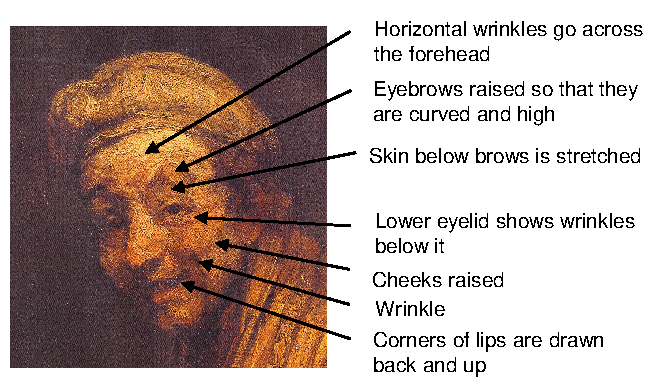
\includegraphics{profUteKunzmann-fig2}}
    \caption{Emotional expressions in paintings: An expert-based approach}
    \label{fig2:profUteKunzmann}
  \end{center}
\end{figure}

The consensus-based approach to describing emotional expressions in paintings is illustrated through the same self-portrait of Rembrandt (see Figure \ref{fig3:profUteKunzmann}). 

\begin{figure}[htb]
  \begin{center}
    \resizebox{0.4\textwidth}{!}{\includegraphics{profUteKunzmann-fig3}}
    \caption{Emotional expressions in paintings: A consensus-based approach.}
    \label{fig3:profUteKunzmann}
  \end{center}
\end{figure}

This approach is based on laypeople's intuitive understanding of emotions. In a pilot study, young and old laypeople were asked to evaluate the painting in terms of which emotions are depicted. Results supported the expert-based codings and revealed that Rembrandt expresses moderate happiness blended with slight surprise. However, there was also high consensus among laypeople that Rembrandt was mischievous and somewhat ironic. The latter two affective states are not part of Ekman's coding system.

\paragraph{Collaborations}
\begin{itemize}
\item University of Fribourg \\ Caroline Schuster Cordone
\end{itemize}

\paragraph{Grants}

\begin{itemize}
\item Maxnet Aging, Max Planck Society (Start 2007). (PI : U. Kunzmann): Expression of emotions in Art: Art Historical and Psychological Perspectives.
\end{itemize}